\documentclass{ximera}
\graphicspath{     %% setup a global graphics path
{./}               %% look in the same-level directory
{./pictures/}      %% look in graphics
{../pictures/}     %% look up one directory, then in graphics
%{../../pictures/} %% look up two directories, then in graphics
}

\author{Zack Reed}
%borrowed from selinger linear algebra
\title{Definitions, Theorems, Formulas, and More}

\begin{document}
\begin{abstract}

\end{abstract}
\maketitle

While reading through a textbook and gaining new tools, such as definitions, theorems, and formulas, progressively as the content is presented is very important. It can, however, make it hard to reference these tools outside of specific chapter or section contexts when needed for problem solving.

Here is a list of all relevant definitions, theorems, formulas, and other information that you might want to have on hand while you do homework and problem solve.

The content is organized by topic (as much as possible): 1) vectors, 2) matrices, 3) vector spaces. If you have trouble finding a particular bit of information, try first searching according to how it's used (e.g. to help with vectors, matrices, vector spaces, etc.). Also, there is likely more content here than is presented in the Learning Activities, feel free to use whatever tools you have available to solve problems, but the problems will only need the material from the Learning Activities.

\section{Vectors}

\begin{definition}{Scalars}\label{def:scalars1}

    For now, we're going to think of \textbf{scalars} as real numbers. $1$, $100$, $\pi$, $e^2$, are all examples of scalars.

\end{definition}

\begin{definition}\name{Tuples}\label{def:tuples}
We can organize the measurements of the apple by encoding values of the apple's useful features as the locations in space. This is what's called a tuple, or more specifically an \textit{ordered tuple}. We more colloquially call these \textit{points} in space, however depending on the context you can equally call them \textit{vectors}.
\end{definition}


\begin{definition}\name{Ordered Pairs}\label{def:orderedpairs}
    An ordered pair is just a pair of numbers $[a,b]$ delineated by parenthesis (or brackets) with the entries separated by a comma. It's called ``ordered'' because $[a,b] \ne [b,a]$. 
    
\begin{example}

      In terms of vectors, if $\vec{v}=[3,4]$ and $\vec{w}=[4,3]$, then $\vec{v}\ne \vec{w}$, because the first coordinate of $\vec{v}$ is $3$ and the first coordinate of $\vec{w}$ is $4$.

\end{example}
    
    \item[An ordered tuple] is just an array (i.e. a list) of an arbitrary, but fixed, number of elements that is ordered like an ordered pair. As before, while some might want to only call these \emph{points} in space, it is often equally useful to just call them \emph{vectors}.
    
    \item[Coordinates:] Each position in the array (e.g first, second, third) is called a \textit{coordinate}. In the vector $[a, b, c]$, we say that $a$ is the first coordinate, $b$ is the second coordinate, and $c$ is the third coordinate. 

\end{definition}

\begin{definition}\name{The position vector}\label{def:posvec}

    Let $P$ be a tuple location in $n$-dimensional space. The \textbf{position
      vector}%
    \index{position vector} of $P$ is the vector
    $\vec{p}$ whose tail is at the origin and whose tip
    is at $P$.
    \begin{center}
      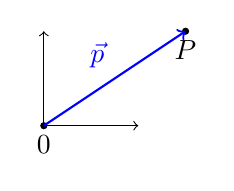
\begin{tikzpicture}[scale=0.6]
        \draw[<->](2,0,0)--(0,0,0)--(0,2,0);
        \draw[fill] (0,0) circle [radius=1.8pt] node[below]{$0$};
        \draw[fill] (3,2) circle [radius=1.8pt] node[below]{$P$};
        \draw[thick, blue, ->](0,0) -- node[above left]{$\vec{p}$} (3,2);
      \end{tikzpicture}
    \end{center}
    If the point $P$ has coordinates $(p_1,\ldots,p_n)$, then the
    components of the position vector are
    \begin{equation*}
      \vec{p} =
      \startmat{c}
        p_1    \\
        \vdots \\
        p_n
      \stopmat.
    \end{equation*}
    Thus, the coordinates of a point are the same as the components of
    its position vector. 
    
    \begin{remark}
    
    For this reason, we will often interchangeably visualize vectors as points in space, or visualize them as arrows. For the purposes of this course, the choice of one over the other is often cosmetic, or a matter of emphasis. If there are too many vectors to nicely visualize at once as arrows, we'll often use points instead.

  \end{remark}
  \end{definition}

\begin{definition}{Vectors as Addition and Scalar Multiplication}\label{def:vecasaddmult}

    Vectors, thought of most abstractly, are quantities where addition and scalar multiplication make sense. We'll get more precise about this later, but for now we're going to call a collection of vectors a \textit{vector space} if for $\vec{v}$ and $\vec{w}$ in the space, $a\vec{v}+b\vec{w}$ is also in the space for all scalars $a$ and $b$. We would call $\vec{v}$ and $\vec{w}$ \textit{vectors}.

\end{definition}

\begin{definition}\name{Distance between points}\label{def:distpoints}
  
    Let $P=(p_1,\ldots,p_n)$ and $Q=(q_1,\ldots,q_n)$ be two points in
    $\R^n$. Then the \textbf{distance}%
    \index{distance!point to point} between these points is defined as
    \begin{equation*}
      d(P, Q) = \sqrt{(p_1-q_1)^2 + \ldots + (p_n-q_n)^2}.
    \end{equation*}
    This formula is also called the \textbf{distance formula}%
    \index{distance formula}. We may also write $\left\|PQ\right\|$ for the
    distance between $P$ and $Q$.
\end{definition}

\begin{definition}\name{Length of a vector}\label{def:veclength}
    Let
    \begin{equation*}
      \vec{u} = \startmat{c} u_1 \\ \vdots \\ u_n \stopmat
    \end{equation*}
    be a vector in $\R^n$. Then the \textbf{length}%
    \index{vector!length}%
    \index{length of a vector} of $\vec{u}$, written $\left\| \vec{u} \right\|$,
    is given by
    \begin{equation*}
      \left\| \vec{u} \right\| = \sqrt{u_1^2 + \ldots + u_n^2}.
    \end{equation*}
    The length of a vector is also sometimes called its
    \textbf{magnitude}%
    \index{magnitude!of a vector}%
    \index{vector!magnitude} or its
    \textbf{norm}%
    \index{norm!in Rn@in $\R^n$}%
    \index{vector!norm}.
\end{definition}

\begin{definition}\name{Unit Vectors}\label{def:unitvec}

    A \textbf{unit vector} is a vector of length $1$. 

    In $\R^n$, the standard coordinate vectors are examples of unit vectors. In $\R^3$, the coordiante vectors are $\vect{i}=[1,0,0]$, $\vect{j}=[0,1,0]$, and $\vect{k}=[0,0,1]$.
\end{definition}

\begin{definition}\name{Scalar Multiplication of a Vector}\label{def:scalarmult}

    Let $\vec{v} = \startmat{c} v_1 \\ \vdots \\ v_n \stopmat$ be a vector in $\R^n$ and let $c$ be a scalar. The \textbf{scalar multiple} of $\vec{v}$ by $c$ is the vector
    \begin{equation*}
      c\vec{v} = \startmat{c} cv_1 \\ \vdots \\ cv_n \stopmat.
    \end{equation*}

\end{definition}

\begin{definition}\label{def:dotproduct}
    Let $\vec{u}$ and $\vec{v}$ be vectors in $\RR^n$.  The \dfn{dot
      product} of $\vec{u}$ and $\vec{v}$, denoted by
    $\vec{u}\dotp \vec{v}$, is given by
    \begin{align*}
      \vec{u}\dotp\vec{v}=\begin{bmatrix}u_1\\u_2\\\vdots\\u_n\end{bmatrix}\dotp\begin{bmatrix}v_1\\v_2\\\vdots\\v_n\end{bmatrix}=u_1v_1+u_2v_2+\ldots+u_nv_n.
    \end{align*}
\end{definition}


\begin{definition}\name{Addition of vectors in $\R^n$}\label{def:vecadd}
    For vectors $\vec{u}=\startmat{c}
      u_1 \\
      \vdots \\
      u_n
    \stopmat,\; \vec{v}= \startmat{c}
      v_1 \\
      \vdots \\
      v_n
    \stopmat$ in $\R^n$, the sum $\vec{u}+\vec{v}$ in $\R^n$ is defined
    by
    \begin{equation*}
      \vec{u}+\vec{v} = \startmat{c}
        u_1 \\
        \vdots \\
        u_n
      \stopmat +  \startmat{c}
        v_1 \\
        \vdots \\
        v_n
      \stopmat
      = \startmat{c}
        u_1+v_1 \\
        \vdots \\
        u_n+v_n
      \stopmat.
    \end{equation*}
  \end{definition}

\section{Matrices}

\section{Vector Spaces}

\begin{definition}{Vectors as Addition and Scalar Multiplication}%\label{def:vecasaddmult}

    Vectors, thought of most abstractly, are quantities where addition and scalar multiplication make sense. We'll get more precise about this later, but for now we're going to call a collection of vectors a \textit{vector space} if for $\vec{v}$ and $\vec{w}$ in the space, $a\vec{v}+b\vec{w}$ is also in the space for all scalars $a$ and $b$. We would call $\vec{v}$ and $\vec{w}$ \textit{vectors}.

\end{definition}

\end{document}